\chapter{Configuración y mantenimiento de \ReplicaNextLong{}}\label{ch:replica-next-setup}

Esta sección se aplica al cuadro \ReplicaNextLong{} mostrado en \autoref{fig:next-hardware}.

\begin{figure}[htbp]
    \centering
    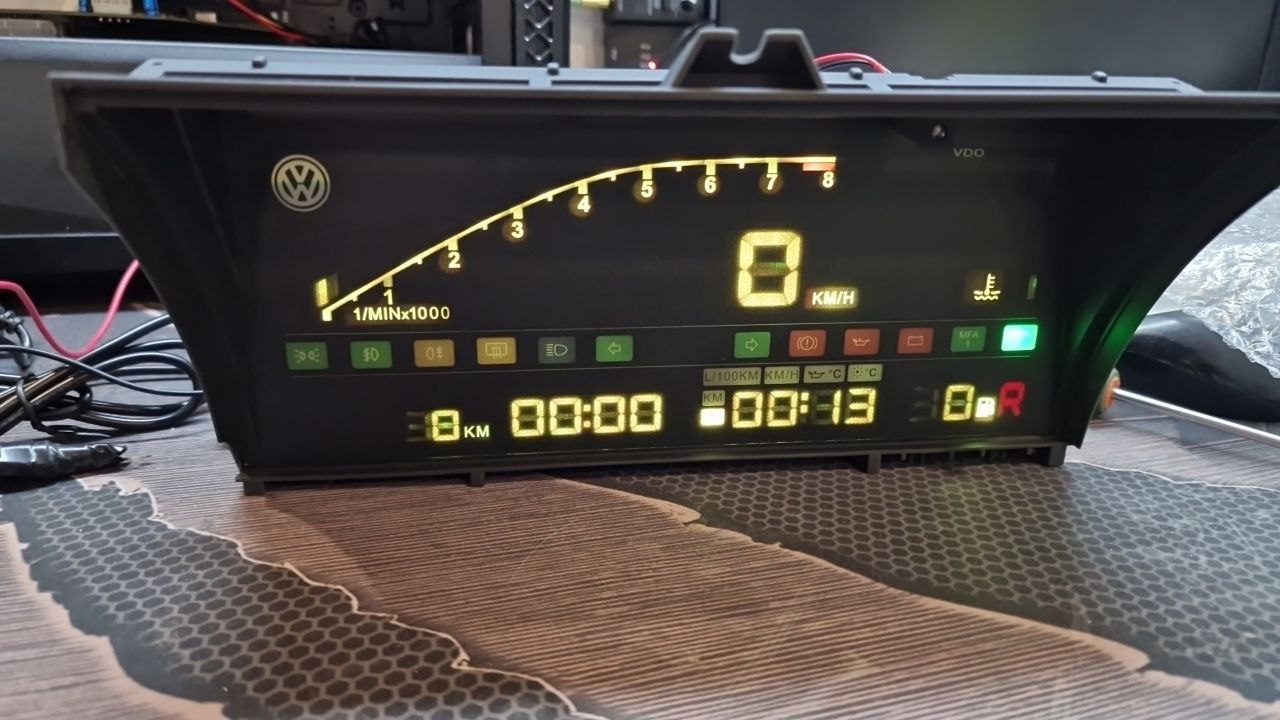
\includegraphics[width=0.6\textwidth]{digifiz_manual/image019.png}
\caption{Conjunto del cuadro \ReplicaNextLong{}.}
    \label{fig:next-hardware}
\end{figure}

\section{Manipulación del panel}
\begin{itemize}
    \item La placa frontal de policarbonato impresa en UV debe protegerse de arañazos y objetos extraños. Los daños considerables requieren piezas de repuesto de PHOL-LABS Kft y no se tratan como un caso de garantía.
    \item El reloj en tiempo real se configura mediante el panel de control Wi-Fi. Se reinicia cada vez que se desconecta la alimentación permanente.
\end{itemize}

\section{Portal de control Wi-Fi}
La configuración, la recopilación de datos y la gestión del firmware se realizan a través de la aplicación web integrada.
\begin{itemize}
    \item Conéctese al punto de acceso Wi-Fi del tablero. Desactive los datos móviles y únase a \texttt{Digifiz\_AP} (contraseña \texttt{87654321}); algunas revisiones anuncian \texttt{PHOL-LABS2} con la misma contraseña.
    \item La dirección IP predeterminada es \texttt{192.168.4.1}. Si el cuadro está configurado para unirse a otra red, escanee la subred en busca de una dirección que termine en \texttt{.32} utilizando una aplicación de herramientas IP.
    \item El portal contiene cinco pestañas: \emph{WiFi}, \emph{Control}, \emph{Settings}, \emph{Colors} y \emph{About} (\autoref{fig:next-control-tabs}). La pestaña Wi-Fi configura los ajustes de red y gestiona la carga de firmware; la pestaña Control ajusta los parámetros del cuadro; la pestaña Settings ofrece un editor estructurado para todos los parámetros del firmware; la pestaña Colors gestiona los esquemas de color multisegmento; la pestaña About muestra información de los autores.
\end{itemize}

\begin{figure}[htbp]
    \centering
    \begin{subfigure}{0.48\textwidth}
        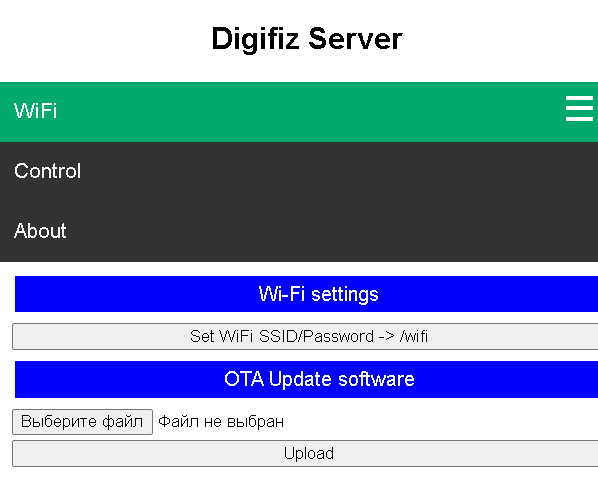
\includegraphics[width=\linewidth]{digifiz_manual/image020.png}
        \caption{Control tab overview.}
    \end{subfigure}\hfill
    \begin{subfigure}{0.48\textwidth}
        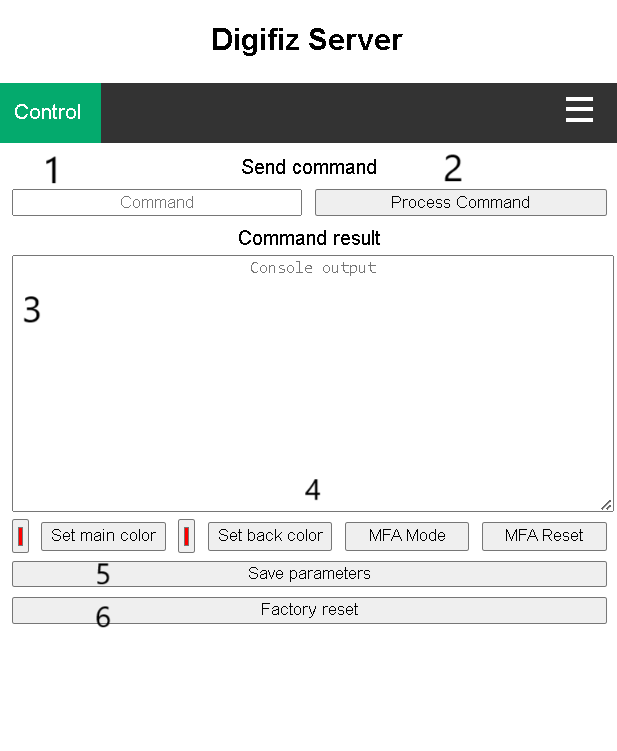
\includegraphics[width=\linewidth]{digifiz_manual/image021.png}
        \caption{Numbered controls and command entry fields.}
    \end{subfigure}
    \caption{Interfaz Wi-Fi de \ReplicaNextShort{}.}
    \label{fig:next-control-tabs}
\end{figure}

\section{Introducción de comandos}
La pestaña \emph{Control} proporciona una línea de entrada de comandos (1), un botón \emph{Process} (2), una ventana de resultados (3), controles rápidos (4), un botón \emph{Save} (5) y un botón \emph{Reset} (6). Introduzca los comandos como pares separados por espacios \verb|<número> <valor>| utilizando únicamente enteros; no se requieren signos de puntuación ni comillas. \autoref{fig:next-command-example} ilustra la interfaz al activar y desactivar el brillo automático.

\begin{figure}[htbp]
    \centering
    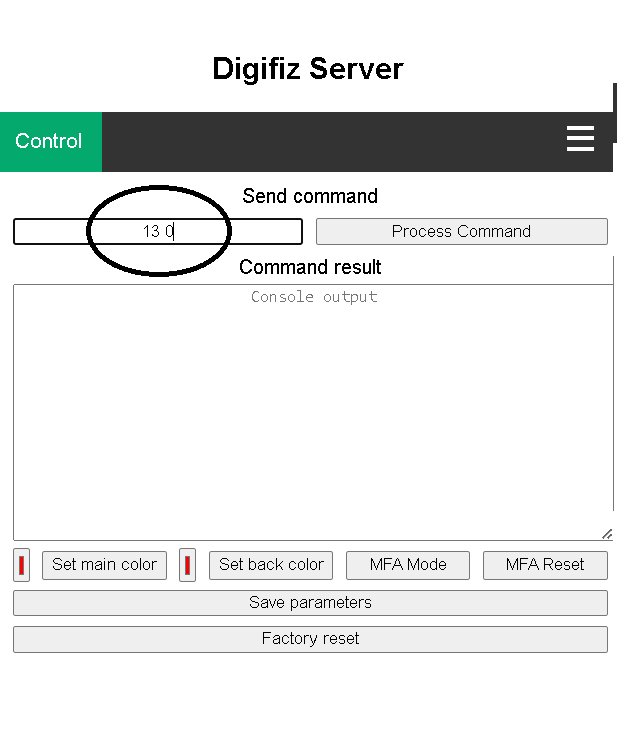
\includegraphics[width=0.55\textwidth]{digifiz_manual/image022.png}
\caption{Ejemplo de secuencia de comandos que desactiva el brillo automático.}
    \label{fig:next-command-example}
\end{figure}

\section{Referencia de comandos}
\begin{table}[htbp]
    \centering
    \caption{Comandos principales de configuración de \ReplicaNextShort{}.}
    \label{tbl:next-commands}
    {\scriptsize
    \begin{tblr}{
        colspec = {Q[c,0.14\linewidth] Q[l,0.36\linewidth] Q[l]},
        rowsep = 2pt,
    }
        \toprule
        \textbf{Comando} & \textbf{Nombre} & \textbf{Descripción} \\
        \midrule
        22 (or 0) & \paramname{PARAMETER\_RPMCOEFFICIENT} & Engine RPM calibration factor (100--10000). \\
        1  & \paramname{PARAMETER\_SPEEDCOEFFICIENT} & Factor de calibración de velocidad (10--255). \\
        2  & \paramname{PARAMETER\_COOLANTTHERMISTORB} & Coeficiente beta del termistor de refrigerante (2000--5000). \\
        3  & \paramname{PARAMETER\_OILTHERMISTORB} & Coeficiente beta del termistor de aceite (2000--5000). \\
        4  & \paramname{PARAMETER\_AIRTHERMISTORB} & Coeficiente beta del termistor ambiente (2000--5000). \\
        5  & \paramname{PARAMETER\_TANKMINRESISTANCE} & Resistencia mínima del aforador (0--1000~\ohm). \\
        6  & \paramname{PARAMETER\_TANKMAXRESISTANCE} & Resistencia máxima del aforador (100--1000~\ohm). \\
        7  & \paramname{PARAMETER\_TAU\_COOLANT} & Constante del filtro de temperatura de refrigerante (1--50; valores altos reaccionan más rápido). \\
        8  & \paramname{PARAMETER\_TAU\_OIL} & Constante del filtro de temperatura de aceite (1--50). \\
        9  & \paramname{PARAMETER\_TAU\_AIR} & Constante del filtro de temperatura ambiente (1--50). \\
        10 & \paramname{PARAMETER\_TAU\_TANK} & Constante del filtro de nivel de combustible (1--50). \\
        11 & \paramname{PARAMETER\_MILEAGE} & Valor total del odómetro (0--999999). \\
        12 & \paramname{PARAMETER\_DAILY\_MILEAGE} & Odómetro parcial (0--9999). \\
        13 & \paramname{PARAMETER\_AUTO\_BRIGHTNESS} & Activar brillo automático (1=activo, 0=desactivado). \\
        14 & \paramname{PARAMETER\_BRIGHTNESS\_LEVEL} & Nivel de brillo manual (0--60\%; valores superiores a 60 reducen la vida del LED). \\
        15 & \paramname{PARAMETER\_TANK\_CAPACITY} & Capacidad del depósito en litros (0--99; 55~L típico en Golf~2). \\
        16 & \paramname{PARAMETER\_MFA\_STATE} & Modo MFA activo (normalmente se controla por hardware). \\
        17 & \paramname{PARAMETER\_BUZZER\_OFF} & Desactivar zumbador (1 lo desactiva, 0 lo habilita; \ReplicaNextShort{} no incluye zumbador). \\
        18 & \paramname{PARAMETER\_MAX\_RPM} & Escala del cuentarrevoluciones (típico 8000, rango 4000--16000). \\
        19 & \paramname{PARAMETER\_NORMAL\_RESISTANCE\_COOLANT} & Resistencia del sensor de refrigerante a \SI{25}{\celsius} (1000--10000~\ohm). \\
        20 & \paramname{PARAMETER\_NORMAL\_RESISTANCE\_OIL} & Resistencia del sensor de aceite a \SI{25}{\celsius} (1000--10000~\ohm). \\
        21 & \paramname{PARAMETER\_NORMAL\_RESISTANCE\_AMB} & Resistencia del sensor ambiente a \SI{25}{\celsius} (1000--10000~\ohm). \\
        23 & \paramname{PARAMETER\_DOT\_OFF} & Comportamiento de los dos puntos del reloj (0=parpadeo, 1=fijo). \\
        24 & \paramname{PARAMETER\_BACKLIGHT\_ON} & Activar retroiluminación con luces de cruce (sin uso en \ReplicaNextShort{}). \\
        25 & \paramname{PARAMETER\_M\_D\_FILTER} & Constante del filtro mediano (heredado, normalmente sin uso). \\
        26 & \paramname{PARAMETER\_COOLANT\_MAX\_R} & Umbral del sensor de refrigerante para indicación a escala completa (\SI{100}{\celsius}--\SI{150}{\celsius}). \\
        27 & \paramname{PARAMETER\_COOLANT\_MIN\_R} & Umbral del sensor de refrigerante para indicación ``1~bar'' (\SI{0}{\celsius}--\SI{80}{\celsius}). \\
        31 & \paramname{PARAMETER\_MAINCOLOR\_R} & Componente roja del color de la interfaz (0--255). \\
        32 & \paramname{PARAMETER\_MAINCOLOR\_G} & Componente verde del color de la interfaz (0--255). \\
        33 & \paramname{PARAMETER\_MAINCOLOR\_B} & Componente azul del color de la interfaz (0--255). \\
        37 & \paramname{PARAMETER\_RPM\_FILTER} & Intensidad del filtro de RPM (10--200; valores altos reaccionan más rápido). \\
        128 & \paramname{PARAMETER\_READ\_ADDITION} & Sumar 128 para leer el valor actual de cualquier comando. \\
        255 & \paramname{PARAMETER\_SET\_HOUR} & Ajustar horas del reloj (formato de 24 horas). \\
        254 & \paramname{PARAMETER\_SET\_MINUTE} & Ajustar minutos del reloj. \\
        253 & \paramname{PARAMETER\_RESET\_DAILY\_MILEAGE} & Restablecer el odómetro parcial. \\
        252 & \paramname{PARAMETER\_RESET\_DIGITAL} & Restablecimiento de fábrica de los parámetros almacenados. \\
        \bottomrule
    \end{tblr}}
\end{table}

\section{Valores predeterminados}
\begin{table}[htbp]
    \centering
    \caption{Valores predeterminados de \ReplicaNextShort{}.}
    \label{tbl:next-defaults}
    {\scriptsize
    \begin{tblr}{
        colspec = {Q[l,0.42\linewidth] Q[c,0.15\linewidth] Q[l]},
        rowsep = 2pt,
    }
        \toprule
        \textbf{Parámetro} & \textbf{Predeterminado} & \textbf{Notas} \\
        \midrule
        \paramname{PARAMETER\_RPMCOEFFICIENT} & 3000 & Típico para entradas de tacómetro Audi. \\
        \paramname{PARAMETER\_SPEEDCOEFFICIENT} & 100 & Calibrado para 100~km/h. \\
        \paramname{PARAMETER\_COOLANTTHERMISTORB} & 4000 &  \\
        \paramname{PARAMETER\_OILTHERMISTORB} & 4000 &  \\
        \paramname{PARAMETER\_AIRTHERMISTORB} & 3812 & 3600 en paneles de segunda generación. \\
        \paramname{PARAMETER\_TANKMINRESISTANCE} & 35 & \ohm. \\
        \paramname{PARAMETER\_TANKMAXRESISTANCE} & 265 & \ohm. \\
        \paramname{PARAMETER\_TAU\_COOLANT} & 2 & Constante del filtro. \\
        \paramname{PARAMETER\_TAU\_OIL} & 2 & Constante del filtro. \\
        \paramname{PARAMETER\_TAU\_AIR} & 2 & Constante del filtro. \\
        \paramname{PARAMETER\_TAU\_TANK} & 2 & Constante del filtro. \\
        \paramname{PARAMETER\_MILEAGE} & Dependiente del vehículo & Mantiene el odómetro almacenado. \\
        \paramname{PARAMETER\_DAILY\_MILEAGE} & 0 &  \\
        \paramname{PARAMETER\_AUTO\_BRIGHTNESS} & 1 & Activado. \\
        \paramname{PARAMETER\_BRIGHTNESS\_LEVEL} & 25 & Predeterminado en generación~2; generación~1/1.5 usa 7 o 13. \\
        \paramname{PARAMETER\_TANK\_CAPACITY} & 63 & Litros. \\
        \paramname{PARAMETER\_MFA\_STATE} & 0 & Página MFA predeterminada. \\
        \paramname{PARAMETER\_BUZZER\_OFF} & 1 & Zumbador desactivado. \\
        \paramname{PARAMETER\_MAX\_RPM} & 8000 & Escala del cuentarrevoluciones. \\
        \paramname{PARAMETER\_NORMAL\_RESISTANCE\_COOLANT} & 1000 & \ohm{} a \SI{25}{\celsius}. \\
        \paramname{PARAMETER\_NORMAL\_RESISTANCE\_OIL} & 1000 & \ohm{} a \SI{25}{\celsius}. \\
        \paramname{PARAMETER\_NORMAL\_RESISTANCE\_AMB} & 2991 & 500~\ohm{} para sensores de segunda generación. \\
        \paramname{PARAMETER\_DOT\_OFF} & 0 & Dos puntos del reloj parpadeando. \\
        \paramname{PARAMETER\_BACKLIGHT\_ON} & 1 & Retroiluminación habilitada con luces de cruce. \\
        \paramname{PARAMETER\_M\_D\_FILTER} & 65535 & Constante heredada del filtro mediano. \\
        \paramname{PARAMETER\_COOLANT\_MAX\_R} & 120 & \si{\celsius}. \\
        \paramname{PARAMETER\_COOLANT\_MIN\_R} & 60 & \si{\celsius}. \\
        \paramname{PARAMETER\_MAINCOLOR\_R} & 180 & Valor por defecto amarillo verdoso. \\
        \paramname{PARAMETER\_MAINCOLOR\_G} & 240 & Valor por defecto amarillo verdoso. \\
        \paramname{PARAMETER\_MAINCOLOR\_B} & 6 & Valor por defecto amarillo verdoso. \\
        \paramname{PARAMETER\_RPM\_FILTER} & 70 & Respuesta del filtro. \\
        \paramname{PARAMETER\_UPTIME} & 0 & Contador de funcionamiento. \\
        \bottomrule
    \end{tblr}}
\end{table}

\section{Lectura de parámetros y ejemplos}
Para leer un parámetro, sume 128 al número de comando (por ejemplo, \verb|129 0| devuelve el coeficiente de velocidad). Entre los comandos habituales se incluyen desactivar el brillo automático (\verb|13 0|), activarlo de nuevo (\verb|13 1|), ajustar el coeficiente de velocidad (\verb|1 110| incrementa en un 10\% la velocidad mostrada) y fijar el odómetro (\verb|11 123456|). Los valores del reloj se ajustan con \verb|255 <horas>| seguido de \verb|254 <minutos>|. Los comandos 31--33 establecen los componentes RGB del color de la interfaz.

\section{Comandos de servicio}
Las revisiones recientes del firmware aceptan nombres de parámetros legibles, por ejemplo \verb|PARAMETER_RPMCOEFFICIENT 3000|. El comando de diagnóstico \verb|adc 0| muestra lecturas ADC sin procesar para diagnosticar sensores. Las actualizaciones de firmware añaden controles visuales de color, por lo que conviene actualizar periódicamente desde la pestaña \emph{WiFi} para acceder a las últimas funciones.

\section{Editor de parámetros en la pestaña Settings}
La pestaña \emph{Settings} refleja la lista de parámetros de \autoref{tbl:next-commands} y \autoref{tbl:next-defaults} e incorpora metadatos sobre rangos, descripciones y tipos de datos.
Utilícela cuando prefiera un flujo de trabajo gráfico en lugar de introducir números de comando.

\begin{enumerate}
    \item Pulse \emph{Load Parameters} para obtener los valores en vivo del cuadro. El navegador muestra cada elemento con su nombre, valor actual, descripción emergente y tipo.
    \item Para las entradas numéricas, escriba el valor deseado en la columna \emph{New Value}. La interfaz aplica el rango permitido mostrado en las columnas \emph{Min} y \emph{Max}. Los parámetros booleanos aparecen como casillas de verificación.
    \item Haga clic en \emph{Set} para enviar el cambio al instante. La tabla se actualiza para confirmar el valor modificado.
    \item Repita el proceso para cada parámetro que desee ajustar. Cuando termine, vuelva a la pestaña \emph{Control} y pulse \emph{Save parameters} para guardar la configuración en la memoria no volátil.
\end{enumerate}

El flujo de trabajo de colores exige habilitar la marca de firmware responsable de las paletas personalizadas antes de ir a la pestaña \emph{Colors}.
Busque la entrada booleana denominada “Custom colour scheme” (publicada como \verb|PARAMETER_CUSTOM_COLORSCHEME_ENABLE| en la lista de parámetros), marque la casilla y pulse \emph{Set}. El cuadro rechazará modificaciones personalizadas de segmentos hasta que esta marca esté activada.

\section{Esquemas de color personalizados}
La pestaña \emph{Colors} incorpora un editor por segmentos para la retroiluminación LED WS2812. Cada fila describe un punto final del rango, el área funcional correspondiente y el color o la herencia de un color base.

\begin{enumerate}
    \item Pulse \emph{Load Scheme} para leer el mapeo activo. Utilice \emph{Add Segment}, o los controles integrados ``+\textuparrow{}'' y ``+\textdownarrow{}'', para insertar nuevos rangos. Los menús desplegables seleccionan la función del instrumento y el selector de color base permite reutilizar los colores principal o de fondo en lugar de definir un valor RGB fijo.
    \item Haga clic en el selector de color para ajustar el tono RGB de los segmentos configurados como ``Custom''. El editor muestra los valores de los componentes en tiempo real.
    \item Use las flechas de reordenación para que coincida la secuencia física de los LED (los segmentos deben permanecer en orden ascendente). Elimine filas redundantes con el botón ``\texttimes{}''.
    \item Cuando la tabla refleje la distribución deseada, pulse \emph{Set Scheme}. El navegador recorre las filas y envía cada segmento al cuadro.
    \item Cambie inmediatamente a la pestaña \emph{Control} y pulse \emph{Save parameters}. Este paso es obligatorio: el firmware almacena los segmentos cargados en la RAM y los descarta tras un reinicio si no se guardan.
    \item Opcionalmente exporte la representación JSON mediante \emph{Export to File} para crear copias de seguridad, o importe un archivo guardado previamente con \emph{Import from File}. El botón \emph{Reset Scheme} restaura el diseño de fábrica tras confirmar la acción.
\end{enumerate}

Si posteriormente desactiva la marca de esquemas de color personalizados en la pestaña \emph{Settings}, el cuadro volverá al modo clásico de color único controlado por \verb|PARAMETER_MAINCOLOR_R/G/B|.
